\section{Thermal Expansion}


%Solids (bimetallic strip)

\subsection{Expansion of Solids: Screw and Loop}
\begin{itemize}
\item{Preparation Time: 5 minutes}
\item{Materials: screw, length of thick-ish metal wire about 10 cm, heat source, tongs}
\item{Procedure: Bend the wire into a loop such that the head of the screw will just fit through. Demonstrate that the screw fits, then heat the screw in a candle or jiko for a minute or so. Try to pass the screw through the loop again; demonstrate that it no longer fits! Try alternately heating the loop and screw, then let them cool and see if the screw fits again.}
\item{Theory: Metals expand when heated. When you heat the screw, the diameter of the head increases slightly. It is not noticeable to the naked eye, but it becomes obvious when the screw becomes too large to fit into the loop.}
\end{itemize}


\subsection{Thermal Expansion of Solids - Breaking Glass}

\subsubsection*{Learning Objectives}
\begin{itemize}
\item{To observe the effects of thermal expansion of solids}
\item{To break glass containers evenly}
\end{itemize}

\subsubsection*{Background Information}
Solids expand when heated, though not always noticeably.  However, it is enough that if an object is heated on one side but not on another, the side that is heated expands and the other side does not.  If the object is rigid, like glass, it will break instead of bending.  In this way, glass containers like soda bottles and beakers can be broken evenly.

\subsubsection*{Materials}
Soda bottle or other open glass container (bottles with uniform sides are best), water, heat source

\subsubsection*{Hazards and Safety}
\begin{itemize}
\item{The glass will break and may leave sharp edges.  It is important that the glass is properly disposed of.}
\item{Be sure that the bottle is not covered.  If you cover the bottle it could explode rather than just break evenly.}
\end{itemize}

\subsubsection*{Preparation Procedure}
\begin{enumerate}
\item{Collect all materials.}
\end{enumerate}

\subsubsection*{Activity Procedure}
\begin{enumerate}
\item{Place some water in the soda bottle so that it is about half full.  It is best if the water level is at a point where the bottle's side is uniform.}
\item{Place the bottle over a heat source and wait.}
\item{If the bottle does not break before the water boils, remove the bottle from the heat until the water stops boiling, then place it in a container of cold water.}
\end{enumerate}

\subsubsection*{Results and Conclusions}
The glass bottle will break evenly at the level of the water inside.  This is because the water is gaining more heat than the air above it, so the glass bottle touching the water gains more heat than the glass touching the air.  Therefore the glass below the water level expands more than the glass above the water level, so the glass breaks evenly.

\subsubsection*{Clean Up Procedure}
\begin{enumerate}
\item{Dispose of broken glass.}
\item{Return all materials to their proper places.}
\end{enumerate}

\subsubsection*{Discussion Questions}
\begin{enumerate}
\item{Why does the bottle break at the level of the water?}
\item{Which part of the glass bottle is expanding most?}
\end{enumerate}

\subsubsection*{Notes}
Glass is one of the few materials which does this.  Metal bends when heated, hence the bimetallic strip.  However, a similar technique is used in many places to break large stones, especially in villages where other equipment is not available.


\subsection{Bimetallic Strip}

\subsubsection*{Learning Objectives}
\begin{itemize}
\item{To identify components of a bimetallic strip} 
\item{To observe and explain the function of a bimetallic strip} 
\item{To understand the mode of action of a bimetallic strip} 
\end{itemize}

\subsubsection*{Background Information}
Solids expand when heated, but every solid has a different expansivity which depends on what material it is. For example, copper expands noticeably when heated, but wood barely expands at all.  

\subsubsection*{Materials}
Aluminium foil, paper, glue, candle, matches

\begin{figure}
\begin{center}
%\def\svgwidth{150pt}
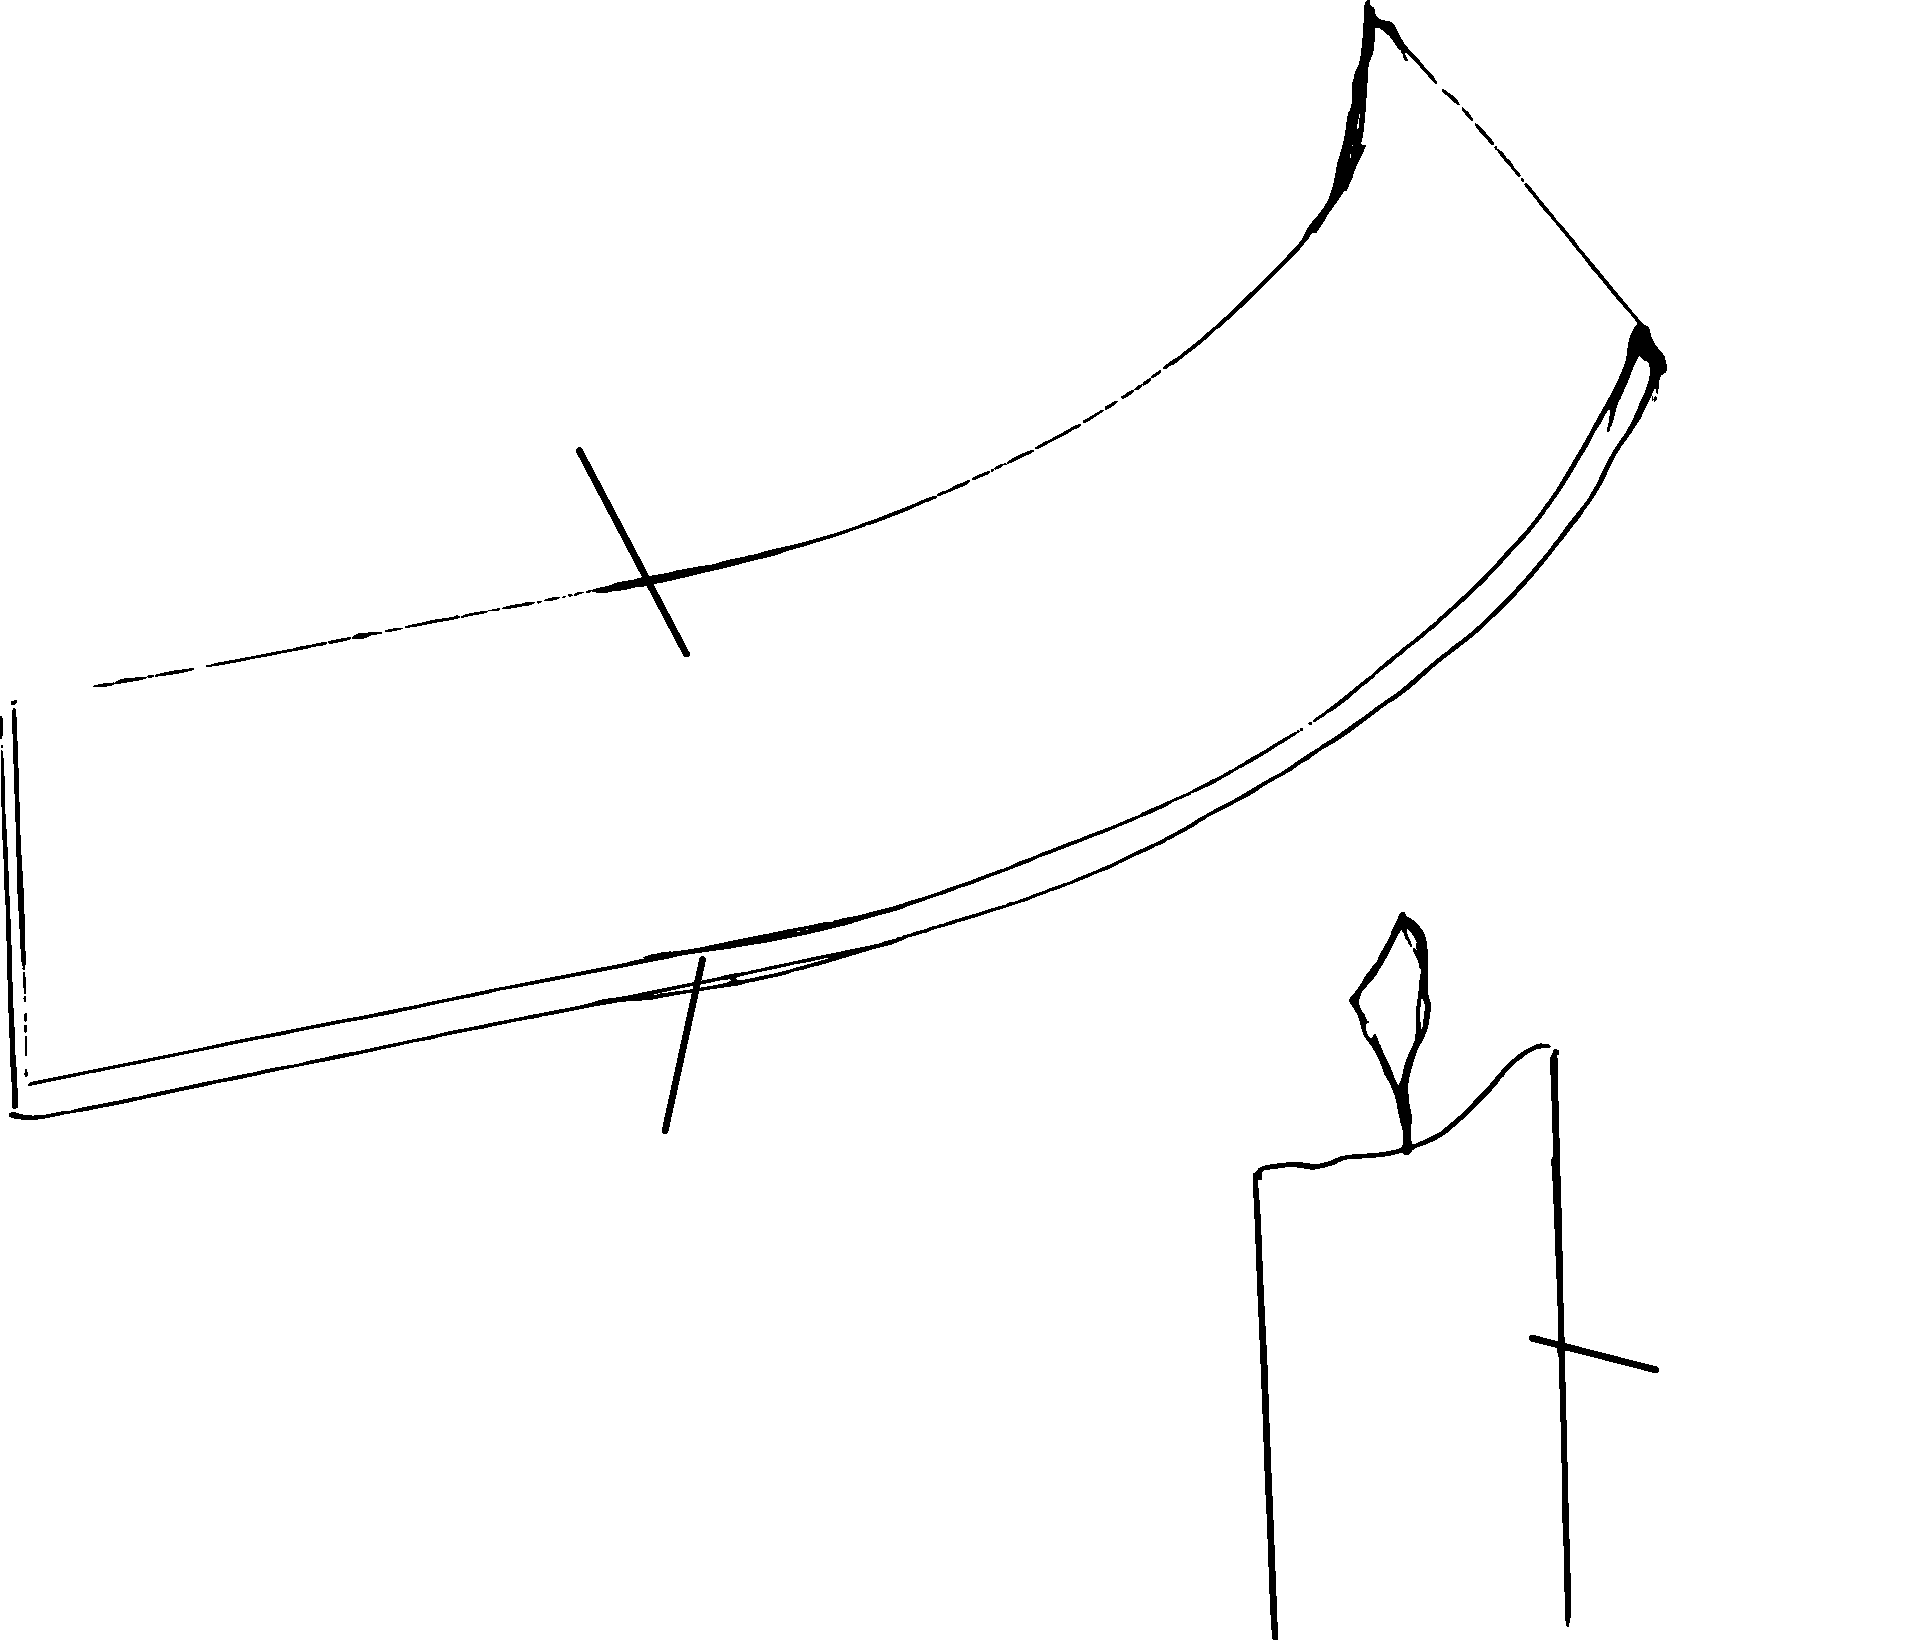
\includegraphics{./img/bimetallic-strip.png}
\caption{A Bimetallic Strip}
\label{fig:bimetallic-strip}
\end{center}
\end{figure}

\subsubsection*{Preparation Procedure}
\begin{enumerate}
\item{Cut one piece of aluminium foil and one piece of paper of equal size. About 3 cm by 10 cm works well.} 
\item{Lay the foil flat on the paper so that they are aligned.} 
\item{Glue the pieces together and leave them to dry.} 
\end{enumerate}

\subsubsection*{Activity Procedure}
\begin{enumerate}
\item{Light the candle.} 
\item{Hold the strip above the candle far enough away that it won't burn or blacken, but close enough that it can feel the heat of the flame.} 
\item{Observe any changes in the shape of the strip.} 
\end{enumerate}

\subsubsection*{Results and Conclusions}
The strip bends towards the side of the paper because the aluminium foil expands more than the paper, forcing the paper to bend in to accommodate the expanding foil.  

\subsubsection*{Clean Up Procedure}
Snuff the candle and return all materials to their proper places.

\subsubsection*{Discussion Questions}
\begin{enumerate}
\item{What happens when the strip is held above the flame with the paper on the bottom and foil on top?}
\item{What happens when the strip is held above the flame with the foil on the bottom and paper on top?}
\item{Why does this occur?}
\end{enumerate}

\subsubsection*{Notes}
A real bimetallic strip contains two metals: usually copper and iron or two other strong metals. The metals, as with the paper and foil, have different expansivities. When they are heated, the metal with the larger expansivity expands more than the other. But as they are attached along their lengths, the more expansive metal pulls the other metal and therefore bends inward toward the metal with lower expansivity.  
In this activity, the paper acts as the metal with lower expansivity, bending inward to accommodate the expanding foil while note expanding much itself.  
It helps in this activity to hold just a piece of foil or piece of paper over the flame first to show that, alone, neither one will bend. They only bend when they are glued together.


\subsection{Thermal Switch}

\subsubsection*{Learning Objectives}
\begin{itemize}
\item{To observe the thermal expansion and contraction of solids} 
\item{To explain the mode of action of a thermal switch} 
\item{To explain the effect of heating on solids} 
\end{itemize}

\subsubsection*{Background Information}
All substances expand when heated. Solids expand only a small amount, but metals expand noticeably.  

\subsubsection*{Materials}
flat piece of wood, 2 thick sticks about 5 cm tall, several small nails, short piece of thick wire (about 8 cm), connecting wires, 2 dry cells, bulb or galvanometer, candle, matches

\subsubsection*{Hazards and Safety}
\begin{itemize}
\item{The thick wire will become very hot in the candle, so be sure not to touch it.} 
\end{itemize}

\subsubsection*{Preparation Procedure}
\begin{enumerate}
\item{Collect all materials.} 
\item{Nail the two sticks upright on the piece of wood, about 6 cm apart.} 
\item{Fix one nail into the side of one stick near the top so that it sticks out horizontally towards the other stick.} 
\item{Bend the end (about half a cm) of the wire at a right angle.} 
\item{Place the wire on the top of the other stick so that the bent end just touches the nail fixed to the other stick.} 
\item{Move the wire back slightly so that there is a gap of about 1 mm between the bent end of the wire and the nail.} 
\item{Fix the wire where it is by putting a nail in the top of the stick to hold the wire in place.} 
\item{Attach one connecting wire to the back of the thick wire and the other connecting wire to the nail fixed to the top of the other stick.} 
\item{Attach the connecting wires to the bulb and batteries in series.} 
\item{You should now have a circuit in series which is disconnected by the small gap between the thick wire and the nail.} 
\end{enumerate}

\begin{figure}
\begin{center}
\def\svgwidth{150pt}
\input{./img/thermal-switch.pdf_tex}
\caption{A Thermal Switching Circuit}
\label{fig:thermal-switch}
\end{center}
\end{figure}

\subsubsection*{Activity Procedure}
\begin{enumerate}
\item{Set up the switch circuit on the table.} 
\item{Check to make sure that the batteries and bulb are working and that there is a small gap between the thick wire and the nail.} 
\item{Light the candle.} 
\item{Hold the candle under the thick wire until the wire expands to touch the nail. The bulb should light.} 
\item{Take the candle away to let the wire cool. The bulb should turn off.} 
\item{Repeat these steps until it is clear what is causing the bulb to turn on and off.} 
\end{enumerate}

\subsubsection*{Results and Conclusions}
The wire's length increases when it is in the candle flame and decreases when the candle is removed and the wire is allowed to cool. This is because the wire (a solid) expands when it is heated. This application of thermal expansion is used in thermostats.  

\subsubsection*{Clean Up Procedure}
Disconnect all wires and return all materials to their proper places.

\subsubsection*{Discussion Questions}
\begin{enumerate}
\item{What happens to the wire when it is heated? What happens when it is cooled?}
\item{What causes the circuit to be completed and the bulb to turn on?}
\item{What causes the bulb to turn off?}
\end{enumerate}

\subsubsection*{Notes}
Solids typically expand very little so that it is difficult to see with the naked eye. Metals expand enough that they can be used to demonstrate thermal expansion. The wire in this activity expands in the candle flame to complete the circuit, thereby lighting the bulb. When the source of heat is removed, the metal cools quickly and contracts, breaking the circuit and turning off the bulb.

%Liquids

%\subsection{Expansion of Liquids: Moving Colors}
%\begin{itemize}
%\item{Preparation Time: 15 minutes}
%\item{Materials: 0.5 liter water bottle, water, food coloring, metal pot, heat source, straw, knife, glue}
%\item{Procedure: Cut a small hole in the bottle cap for the straw to fit through. Insert the straw most of the way and glue it so that it is airtight. Fill the bottle most of the way with water and add some food coloring, then close the cap. Place the bottle into a metal pot with more water and heat the metal pot. As the temperature increases, the level of colored water in the straw will increase. When the level is high enough and the students can see clearly what is happening, take the bottle out of the metal pot and dip it in cold water. Watch the level in the straw drop quickly!}
%\item{Theory: As with solids and gases, liquids expand when heated. In a sealed bottle with a straw, the liquid must expand as the temperature increases and can only move up the straw.}
%\end{itemize}


\subsection{Thermal Expansion of Liquids}

\subsubsection*{Learning Objectives}
\begin{itemize}
\item{To observe the expansion of liquids when heated} 
\item{To observe that different liquids expand at different rates} 
\end{itemize}

\subsubsection*{Background Information}
All substances expand when heated. While solids expand with specific dimensions, liquids and gases expand in volume only.  

\subsubsection*{Materials}
500 mL plastic water bottle with cap, nail, source of heat, small cooking pot, water, food colouring (optional), clear plastic straw or tubing, super glue, various liquids (cooking oil, kerosene, milk, etc.  )

\subsubsection*{Hazards and Safety}
\begin{itemize}
\item{The water in the small pot will boil after a short time, so be careful not to touch it.} 
\end{itemize}

\subsubsection*{Preparation Procedure}
\begin{enumerate}
\item{Collect all materials.} 
\item{Heat the nail.} 
\item{Use the hot nail to put a hole through the center of the bottle cap.} 
\item{Insert the straw through the hole half way so that half of the straw is below the cap and half is above.} 
\item{Use the hot nail and super glue to seal the hole so that no air can pass through the bottle cap. Be careful not to seal the straw itself.} 
\end{enumerate}

\subsubsection*{Activity Procedure}
\begin{enumerate}
\item{Fill the bottle three quarters with water and add a pinch of food colouring.} 
\item{Close the cap on the bottle so that the bottom of the straw is in the water.} 
\item{Fill the small pot half way with water.} 
\item{Place the pot over the heat source and place the water bottle in the pot (water bath).} 
\item{Allow the water to heat and observe the water level in the straw.} 
\item{Remove the water bottle from the pot and place it in cold water.} 
\item{Observe again the water level in the straw.} 
\item{Repeat all of these steps for various other liquids.} 
\item{If possible, prepare one water bottle for each liquid and observe their levels at the same time in the water bath.} 
\end{enumerate}

\subsubsection*{Results and Conclusions}
Liquids expand when heated and contract when cooled. This is because their atoms are moving with more energy and so must increase in volume. Because the water is sealed in the bottle and is expanding, it can only move up the straw.  

\subsubsection*{Clean Up Procedure}
\begin{enumerate}
\item{Turn off the heat source.} 
\item{Empty all the water and return all materials to their proper places.} 
\end{enumerate}

\subsubsection*{Discussion Questions}
\begin{enumerate}
\item{What happens to the water level in the straw when the water is heated?}
\item{What happens to the water level in the straw when the water is cooled?}
\item{What causes the water level to rise and fall?}
\item{Which liquid expands the fastest?}
\item{Which liquid expands the slowest?}
\end{enumerate}

\subsubsection*{Notes}
Liquids expand noticeably when heated so it is simple to see the effect. By using a capillary tube, we can see the effect much more easily as the liquid level will rise in the tube only. By sealing the cap on the bottle, we allow the liquid to expand in only one direction: up through the capillary tube.  

%Gases

%\subsection{Expansion of Gases: Oil Elevator}
%\begin{itemize}
%\item{Preparation Time: 15 minutes}
%\item{Materials: bottle with cap or flask with stopper, cooking oil, straw, glue}
%\item{Procedure: Create the same bottle-straw configuration as in the Expansion of Liquids demo, or use a flask with a stopper with a glass tube if you have it. Close the cap tightly and carefully pour a drop of oil into the top of the straw. The oil should stop in the straw before reaching the bottom. Heat the bottle a little and watch the oil drop move back up the straw. If you have a glass flask, you should be able to heat it with just your hands.}
%\item{Theory: Gases respond much more to heat than solids or liquids, and will expand noticeably with even a small amount of heat. By slightly heating the bottle, you raise the temperature, and therefore the pressure, of the air inside. As the pressure increases, the air pushes the oil up the straw.}
%\end{itemize}


\subsection{Thermal Expansion of Gases}

\subsubsection*{Learning Objectives}
\begin{itemize}
\item{To observe the expansion of a gas when heated} 
\item{To explain why gases expand when heated} 
\end{itemize}

\subsubsection*{Background Information}
Unlike solids, gases expand quickly when heated. Because the molecules of a gas are spread out and moving, the volume increases quickly when more energy is added.  

\subsubsection*{Materials}
Source of heat, small cooking pot, water, clear thin plastic straw or tubing

\subsubsection*{Hazards and Safety}
\begin{itemize}
\item{The water will boil and the steam will hurt your hand, so use a long straw and keep your hand out of the way of the steam. Use tongs to help you hold the straw if necessary.} 
\end{itemize}

\subsubsection*{Preparation Procedure}
Collect all materials.

\subsubsection*{Activity Procedure}
\begin{enumerate}
\item{Light the heat source.} 
\item{Fill the small pot half-way with water and place it over the heat.} 
\item{Place one end of the straw or tubing just below the surface of the water.} 
\item{Place your thumb over the other end of the straw and remove it from the water so that a single drop remains in the bottom of the straw.} 
\item{Turn the straw over and remove your thumb so that the water drop moves down to the center of the straw.} 
\item{Place one end of the straw back in the water, leaving the other end open.} 
\item{Observe the motion of the water drop in the straw as the water in the pot is heated.} 
\item{Hold your thumb over the open end of the straw.} 
\item{Remove the straw from the water and insert it into cold water.} 
\item{Remove your thumb and observe again the motion of the water drop in the straw.} 
\end{enumerate}

\subsubsection*{Results and Conclusions}
As the gas in the straw is heated, the water drop rises. This is due to the expansion of the gas below the drop, as the gas can only expand up. It will be seen that as the gas in the straw is cooled, the drop falls. This is due to the contraction of the gas below the drop, as the gas decreases in volume when its temperature decreases.  

\subsubsection*{Clean Up Procedure}
Turn off the heat source and return all materials to their proper places.

\subsubsection*{Discussion Questions}
\begin{enumerate}
\item{Describe the behavior of the drop when the straw is heated.} 
\item{Describe the behavior of the drop when the straw is cooled.} 
\item{What causes the drop to move up the straw?}
\item{What causes the drop to move down the straw?}
\item{What is expanding in this experiment? What is expanding the fastest?}
\end{enumerate}

\subsubsection*{Notes}
The behavior of gases is actually more complicated; gases will expand as much as the pressure will allow.

%	Charles' Law

\subsection{Charles' Law, Part A -- Coin Cap}
\begin{itemize}
\item{Preparation time: 30 minutes}
\item{Materials: 2 coins, 2 bottles, some way to cool the air in one bottle either through refrigerator or ice.}
\item{Procedure: Take a coin and a bottle. Place the coin over the mouth of the bottle so it covers the entire opening. This is the control bottle. In a second bottle, place the bottle coin a refrigerator with the coin next to it. After 25 minutes, the air inside of the bottle cools down. Remove the bottle from the refrigerator and immediately cover with a coin as before. If no refrigeration is available, take some ice water or cold water and pour into the bottle. Swirl and mix the cold water to ensure the bottle is cold. Pour out the water and cover with the coin. Let the two bottles sit next to each other. After a short time, the coin on the refrigerator bottle will be blown off the top.}
\item{Theory: Charles' law states that temperature is directly proportional to volume. As the temperature increases, the volume increases. As temperature decreases, the volume decreases. In this activity, the temperature of the first bottle remains constant so nothing happens. However, the air in the second bottle is at a lower temperature so it has less volume. When the temperature increases, the volume of the air expands in volume. This is shown by the coin being pushed off the lid of the container. The air expands but the coin stands in the way. The air pushes the coin so that it is possible to expand further in volume.}
\end{itemize}

\subsection{Charles' Law, Part B -- Spray Time}
\begin{itemize}
\item{Preparation time: 15 minutes}
\item{Materials: 1 can of non-CFC aerosol spray (e.g. Rungu insect repellent), 1 balloon.}
\item{Procedure: Place the plastic bag or balloon to act as a container over the mouth of the spray container. Use the container and spray it into a balloon. If the balloon is too small, use a funnel. The spray will liquefy and be cold inside the balloon. Tie the balloon. As the liquid warms up to room temperature, it will change from a liquid to a gas. Students should be able to hear and feel it boiling. Further, as the gas heats up, the balloon will expand in size.}
\item{Theory: Charles' Law states that temperature of a gas at constant pressure is directly proportional to volume. Inside of the spray cans, there is a chemical held under high pressure. Phase diagrams show that gases under high pressure become liquids. The pressure is released and the temperature cools. This is called Joule-Thompson effect. It is an adiabatic expansion. However, by spraying long enough the temperature will cool down to the point that the chemicals will change back to a liquid. This liquid can be transferred to the balloon where it changes back into a gas quickly. This is where Charles' Law comes into play. As the gas comes to room temperature, the volume of the trapped gas will increase.\\
This activity also works quite well for showing phase transitions. As liquids change to a gas, they do not disappear. They still exist even though they may not be seen. Here, the liquid changes to a gaseous state, which accompanies the expansion of the balloon. The size of the balloon is the direct representation of the liquid molecules that have evaporated. The mass of the balloon will also be different than that of one filled with normal air.}
\end{itemize}

%\subsection{Charles' Law, Part C -- Bottle Crush}
%\begin{itemize}
%\item{Preparation time: 10 minutes}
%\item{Materials: water bottle, boiling water}
%\item{Procedure: pour some boiling water into the water bottle. Cap the bottle and shake to make sure all the air in the bottle is heated from the hot water. Open the bottle and pour out the liquid. Recap the bottle. After a short time, the bottle will contract.}
%\item{Theory: Charles' law states that volume is proportional to temperature. By capping the hot air inside of the water bottle, the volume of the air inside the bottle will decrease as the temperature of the gas cools off. As the volume of the air reduces, the atmospheric pressure crushes the plastic water bottle.}
%\end{itemize}

\subsection{Egg Suck}
\begin{itemize}
\item{Preparation time: 0 minutes}
\item{Materials: 1 pealed egg, 1 glass bottle with a narrow mouth, like a konyagi bottle, matches, small piece of paper}
\item{Procedure: With the egg ready to cap the alcohol bottle, use a match to light the piece of paper on fire. Drop the paper into the alcohol container. Let it burn for a second, and then cap the bottle with the egg. The egg should be sucked slowly into the bottle if the egg is not too large. If it does not pull into the bottle, you can try again but use petroleum jelly on the mouth. Even if the egg is not sucked into the bottle completely, there will be a suction holding the egg to the bottle. It is possible to lift the bottle by the egg.}
\item{Theory: The burning match and paper heat the air inside the bottle. When we cap the bottle with the egg, we seal the air inside of the bottle. This air sealed inside is at a higher temperature than the surroundings. As the bottle cools down, the pressure of the air inside the bottle decreases. This is a direct example of Charles's law. As the pressure inside drops, the atmospheric pressure still pushes down onto the egg. If pressure difference is sufficient, the egg will be pushed slowly into the bottle.}
\end{itemize}



\subsection{Charles's Law}

\subsubsection*{Learning Objectives}
\begin{itemize}
\item{To observe the relationship between volume and temperature when pressure is constant} 
\item{To explain the meaning of Charles' Law in terms of pressure, volume and temperature} 
\end{itemize}

\subsubsection*{Background Information}
Gases can be measured by three quantities: pressure, volume and temperature. For this reason, we have laws to relate them to each other. When one quantity is held constant, the other two prove to be either directly proportional or inversely proportional.  

\subsubsection*{Materials}
A 5 Litre water bottle with cap, heat source, small cooking pot, water

\subsubsection*{Hazards and Safety}
\begin{itemize}
\item{Be careful when pouring the water from the pot to the bottle. Use a funnel if necessary.} 
\end{itemize}

\subsubsection*{Preparation Procedure}
Collect all materials.

\subsubsection*{Activity Procedure}
\begin{enumerate}
\item{Light the heat source.} 
\item{Fill the small pot with water and place it over the heat source.} 
\item{Allow the water to boil.} 
\item{When the water is boiling, pour it into the water bottle.} 
\item{Close the cap on the bottle and shake the water.} 
\item{Pour the water out of the bottle and close the cap again.} 
\item{Observe any changes to the bottle.} 
\end{enumerate}

\subsubsection*{Results and Conclusions}
After pouring the boiled water into the bottle and closing the cap, the volume of air in the bottle increases.  This is because the air is gaining heat, and therefore kinetic energy, from the water and therefore increasing in volume.  Pouring the water out removes the air's source of heat.  When you replace the cap on the bottle, you return the bottle to a state of constant pressure.  As the air in the bottle cools, the temperature goes down.  Temperature and volume are directly related, so the volume of the bottle decreases.  We see this as the bottle being crushed.

\subsubsection*{Clean Up Procedure}
\begin{enumerate}
\item{Turn off the heat source.} 
\item{Dispose of the water and return all materials to their proper places.} 
\end{enumerate}

\subsubsection*{Discussion Questions}
\begin{enumerate}
\item{What quantity of a gas is constant during this experiment?}
\item{Which two quantities are changing?}
\item{What causes the bottle to be crushed?}
\item{Based on this experiment, what is Charles's Law?}
\end{enumerate}

\subsubsection*{Notes}
Charles's Law states that, when pressure is constant, temperature varies directly with volume. This means that, in an air-tight system, the volume will increase when something is heated or decrease when something is cooled. This is the principle behind thermal expansion and can be seen easily in the thermal expansion demonstrations.  
In this demonstration boiling water is used initially to increases the temperature of the air in the bottle. It is removed and the bottle is sealed, forcing the pressure to remain constant. As the air inside the bottle cools, it decreases the volume, causing the bottle to be crushed from the inside. $T \propto V$ when $P$ is constant.


%	Boyle’s Law

\subsection{Boyle's Law}

\subsubsection*{Learning Objectives}
\begin{itemize}
\item{To observe the relationship between volume and pressure when temperature is kept constant} 
\item{To explain the relationship between pressure and volume} 
\item{To explain Boyle's Law} 
\end{itemize}

\subsubsection*{Background Information}
Gases can be measured by three quantities: pressure, volume and temperature. For this reason, we have laws to relate them to each other. When one quantity is held constant, the other two prove to be either directly proportional or inversely proportional.  

\subsubsection*{Materials}
Syringes without the needle for each student

\subsubsection*{Preparation Procedure}
Collect the syringes and remove the needles.

\subsubsection*{Activity Procedure}
\begin{enumerate}
\item{Pull the syringe plunger back as far as it will go without removing it.} 
\item{Place your thumb over the open end of the syringe.} 
\item{Push the plunger in as hard and as far as you can.} 
\item{Observe any effects.} 
\item{Remove your thumb from the syringe and push the plunger in as far as it will go.} 
\item{Replace your thumb over the opening of the syringe.} 
\item{Pull the plunger out as hard and as far as you can.} 
\item{Observe any effects.} 
\item{Have students try this themselves.} 
\end{enumerate}

\subsubsection*{Results and Conclusions}
It will be seen that as you push the plunger in, there is a strong force pushing both the plunger and their thumb out.  This is the increased pressure of the air inside the syringe.  As you pull the plunger out, there is a strong force pulling both the plunger and your thumb into the syringe. This is the decreased pressure of the air inside the syringe.  As volume is decreased, pressure is increased; as volume is increased, pressure is decreased.  From this we can say that pressure and volume are inversely proportional.  

\subsubsection*{Clean Up Procedure}
\begin{enumerate}
\item{Collect all syringes and return them to their proper place.} 
\end{enumerate}

\subsubsection*{Discussion Questions}
\begin{enumerate}
\item{What quantity is being held constant in this experiment?}
\item{What quantities are changing in this experiment?}
\item{What do you feel on your thumb when you are trying to pull the plunger out? What do you feel when you are trying to push it in?}
\item{Describe the relationship between pressure and volume in this experiment.} 
\item{Based on this experiment, state Boyle's Law.} 
\end{enumerate}

\subsubsection*{Notes}
Pressure varies inversely with volume. As you push the plunger in, you are decreasing the volume and therefore increasing the pressure, which you feel as an outward force.  
As you pull the plunger out, you are increasing the volume and therefore decreasing the pressure, which you feel as an inward force.  


\subsection{Boyle's Law, Part A -- Syringe}
\begin{itemize}
\item{Preparation time: 0 minutes}
\item{Materials: One syringe of any size minus metal needle}
\item{Procedure: Fill the syringe with air until the end of the graduations. Place a finger at the tip of the syringe to create a seal. Press the plunger as far as possible. Make a competition with the students to see which person can decrease the volume the greatest. It should be easy to decrease the volume most of the way but impossible by human means to completely squeeze out the air.}
\item{Theory: Boyle’s law states that the pressure of a gas at a constant temperature is inversely proportional to the volume. As the pressure increases, the volume decreases. As the pressure decreases, the volume increases. As the plunger pushes down on the gas, the volume decreases. As the progressively decreases, the pressure to push the plunger progressively increases. The pressure becomes so great that it is hard to puss the plunger in all the way.}
\end{itemize}

\subsection{Boyle's Law, Part B -- Cartesian Diver}
\begin{itemize}
\item{Preparation time: 5 minutes}
\item{Materials: 1 clear plastic water bottle with cap that forms a good seal, syringe, some weights like small nuts or nails, water}
\item{Procedure: Fill the water bottle completely with water. The water should be at the brim. Place the syringe, with the inside loaded with some weights and some air, carefully in the top of the bottle. The wings on the syringe may need to be cut in order to make the syringe fit through the bottleneck. It might bob out of the top of the bottle a little. Seal the bottle with the cap. Squeeze the bottle. The syringe should sink. Release the pressure and the syringe rises again. If the force required to squeeze the bottle in order to make the syringe sink is too great, there are two things to be done. First, ensure that the water is completely to the brim of the bottle. Second, adjust the size of the bulb on the syringe to minimize the volume of air. Find a new syringe if the syringe leaks water on the inside.}
\item{Theory: An object will float or sink depending on its density relative to the liquid it is in. In this case, if the syringe is less dense than water, it floats. If the density becomes greater than the density of water, it will sink. This is exactly what is happening inside the syringe. Inside, there is some air trapped on the inside. This gas is subject to Boyles’ law. Applying pressure to the bottle increases the pressure pushing on the syringe. This pressure makes the volume of the syringe contract. Since density is defined as the mass over the volume, by squeezing the bottle the density changes. The mass does not change, but the volume of the syringe decreases because the volume of air is compressed. As the volume decreases, the density of the syringe increases. If the density increases sufficiently, the syringe sinks. This is also known as a Cartesian Diver.}
\end{itemize}

\subsection{Boyle's Law, Part C -- Filling a Balloon}
\begin{itemize}
\item{Preparation time: 0 minutes}
\item{Materials: 1 bottle, 1 balloon}
\item{Procedure: First, blow up the balloon to stretch out the balloon and show that there are no holes. Release all air. Stretch the balloon such that it hangs in the bottle. Have students try blow up the balloon inside the bottle. It is impossible for a normal person to fill this bottle.}
\item{Theory: This is another good example of Boyle’s Law. Usually when balloons are used, we think of the gas inside the balloon. However, this time we are concerned with the air inside of the bottle. By filling the balloon, the air of the balloon increases. This means that the volume of the air inside the bottle decreases. In order to decrease the volume of the air inside the bottle, Boyle’s Law says that the pressure needs to increase. The normal human’s lungs cannot blow enough air at a high enough pressure to fill the balloon inside the bottles. }
\end{itemize}

\subsection{Boyle's Law, Part D -- Sucking a Balloon}
\begin{itemize}
\item{Preparation time: 10 minutes}
\item{Materials: balloon, plastic water bottle, straw}
\item{Procedure: In the plastic water bottle, put a straw through part of the wall. Seal it up so that it does not leak air. Place a balloon over the mouth of the bottle so it falls into the bottle. Use the straw to suck air out of the bottle to have the balloon fill with air.}
\item{Theory: As we suck the air out of the bottle, the volume of the air inside of the bottle gets smaller due to Boyle’s Law. The atmospheric pressure compensates by pushing the balloon into the bottle, which fills up with air.}
\end{itemize}

%	Pressure Law
